% cycles per token by operation (names, 50k, seed 0) -- data: sw/zoo/paper_data.py
\pgfplotsset{zoogemv/.style={fill=blue!65!black, draw=none}, zoonorm/.style={fill=orange!80!black, draw=none},
  zooattn/.style={fill=green!50!black, draw=none}, zoorope/.style={fill=green!25, draw=none},
  zooew/.style={fill=orange!35, draw=none}, zooemb/.style={fill=black!25, draw=none}, zoofetch/.style={fill=black!55, draw=none}}
\def\zooproflabels{GPT-2,GRU,RNN}
\def\zooprofn{3}

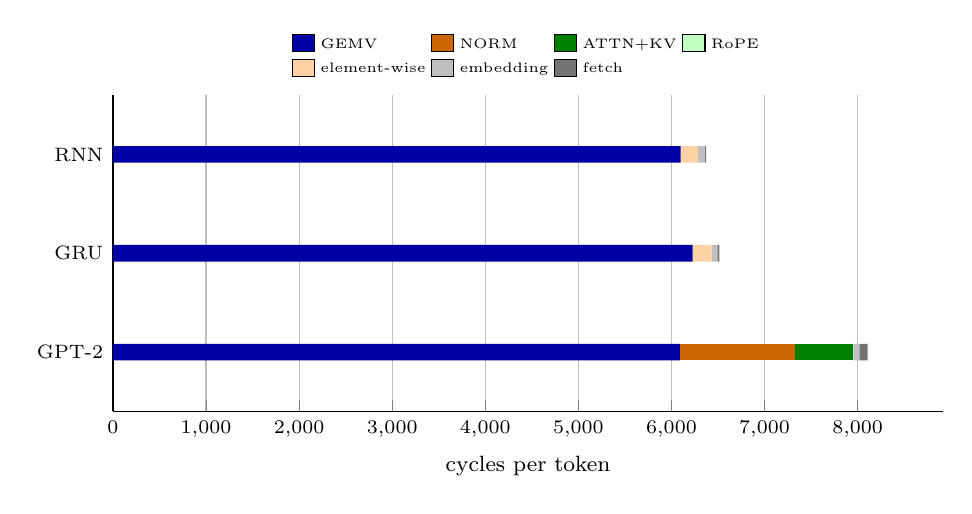
\begin{tikzpicture}
\begin{axis}[xbar stacked, width=\columnwidth, height=5.6cm, bar width=6pt, xmin=0,
  ymin=0.4, ymax=\zooprofn+0.6, ytick={1,...,\zooprofn}, yticklabels/.expand once=\zooproflabels,
  y tick label style={font=\scriptsize}, x tick label style={font=\scriptsize}, xlabel={cycles per token},
  xlabel style={font=\footnotesize}, scaled x ticks=false, xmajorgrids, axis x line*=bottom, axis y line*=left,
  legend style={font=\tiny, at={(0.5,1.02)}, anchor=south, legend columns=4, draw=none}, legend cell align=left]
\addplot[zoogemv] coordinates {(6089.0,1) (6227.0,2) (6099.0,3)};
\addplot[zoonorm] coordinates {(1233.0,1) (0.0,2) (0.0,3)};
\addplot[zooattn] coordinates {(630.9,1) (0.0,2) (0.0,3)};
\addplot[zoorope] coordinates {(0.0,1) (0.0,2) (0.0,3)};
\addplot[zooew] coordinates {(0.0,1) (203.0,2) (184.0,3)};
\addplot[zooemb] coordinates {(66.0,1) (64.2,2) (76.0,3)};
\addplot[zoofetch] coordinates {(89.0,1) (19.0,2) (13.0,3)};

\legend{GEMV, NORM, ATTN+KV, RoPE, element-wise, embedding, fetch}
\end{axis}
\end{tikzpicture}
